\section{Towards Generic Parallel Programming}\label{chap:background}

A programming model exposes constrained semantics to the programmer which that programmer uses to express intent. Absent an embedded programming model, the semantics of C-like languages can lead to sequential thinking and execution. Parallel programming models expose parallel semantics to enable developers to create performance portable code. This is commonly achieved by adding semantic value to the base programming language, often referred to as programming with \emph{pragma} annotations. Other methods expose such semantics through library calls or new languages. All three approaches are conceptually suitable to represent programming paradigms such as tasking, parallel patterns and others. Some representatives are the OpenMP programming model~\cite{CITEOPENMP}, threading libraries, or languages like Erlang in which parallelism is a first-class citizen. In general, it is up to the parallel programming model to expose language constructs or library interfaces (APIs) such that they combine convenience to the programmer with semantics sufficient to map the program execution to the parallel computer hardware efficiently and correctly. 

In designing Kokkos with this mentality, we looked at a broad variety of current and future architectures on which software would need to run. We also looked at our codes, which express many different algorithmic property. We conceived of Kokkos as a generic programming system that could cover the space of architectures we cared about, while exposing semantics in which the algorithms of our codes could be easily expressed. In this way, a generic programming system embedded in the language became the glue between the semantics of a problem domain and the capabilities of an architecture domain.

\begin{figure}
\centerline{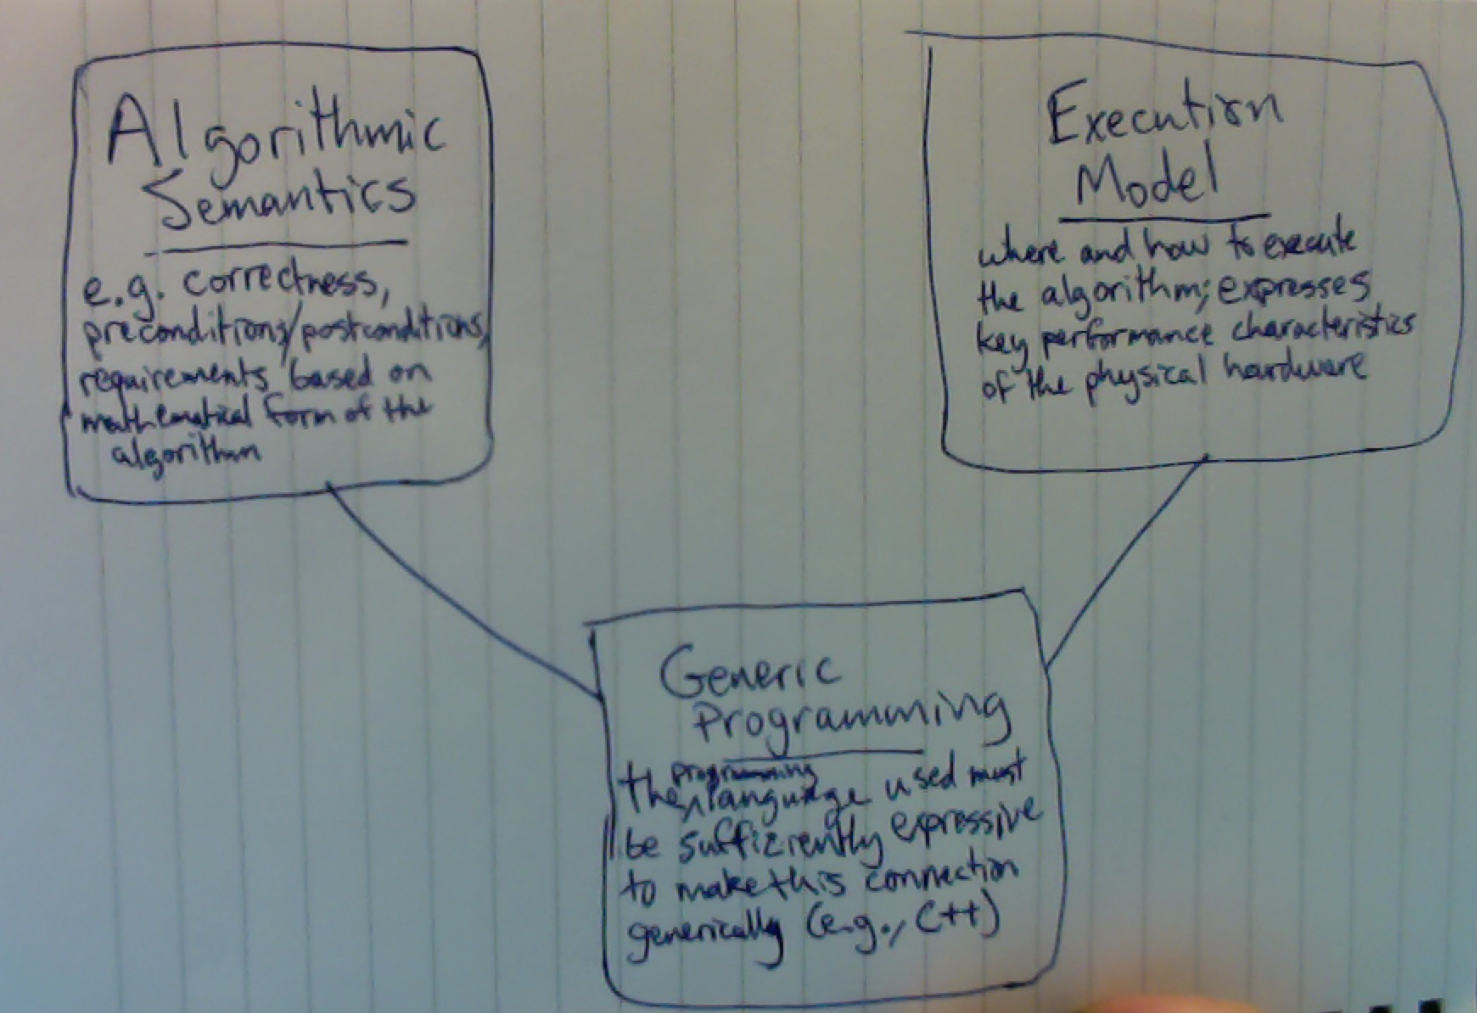
\includegraphics[width=0.45\textwidth]{img/Hollman.png}}
\caption{The Hollman pic :) - placeholder}
\label{fig}
\end{figure}

Earlier we discuss how a programming model constrains semantics to allow the expression of intent in such a way that a developer achieves their goals. Putting together an effective programming model requires constraining semantics such that they enable the necessary parallel paradigms, and expose to users only those aspects of the underlying hardware that they need to think about. We call the combination of constrained semantics, parallel paradigms, and division of responsibility between developer and framework the Semantic Capture.

\begin{figure}[h]
\begin{Verbatim}[frame=leftline]
Constrained Semantics
Parallel Paradigms 
Division of Responsibility
\end{Verbatim}
\caption{Semantic capture - a triplet of constrained semantics, parallel paradigms, and division of responsibilities defined by a parallel programming model to allow developers to run performance-portable code on a set of architectures}
\label{figSemCapture}
\end{figure}

%Semantic information provided by the programmer to the parallel programming model can be grouped into information to express intent and properties. They address the question of \emph{what}, \emph{where} and \emph{how}. In the context of parallel programming, these correspond to defining which code portion to parallelize, where to run and access and how to run that parallel code. Synchronization primitives may be considered as part of the what and information on the execution properties such as data placement or memory access type as the how. Semantics are expressed following a paradigm and a programming language.

To enable developers to achieve performance portability, we needed to constrain what intent they could specify to Kokkos. We settled on Kokkos supporting semantics for offloading loops, the allocation and freeing of data, and data movement. Critically, we decided against exposing machine details to the developer, we aim to increase portability of code by only exposing an abstract execution model (described later) to the users. Our semantics map naturally to C-like languages, with malloc/new calls replaced with the construction and destruction of abstract data types, and many loop types replaced with corresponding parallel patterns. This clean mapping between traditional C-like semantics and our model came from requirements from our physics teams, but also makes Kokkos a good choice for students as it will more closely track with what they've seen before. 

%TODO DZP: keep going here

%The parallel programming paradigm is an abstract ~\emph{representation} with the purpose of facilitating the programmer's understanding of programming rules and program behavior. Which programming paradigm to chose depends on several considerations. Parallel-patterns allow to express concurrency for commonly occurring programming patterns such as loop constructs. Tasking is a paradigm that support the expression of concurrent loops as well as irregular algorithms. Distributed and correctness-oriented programming models may implement actor-based programming. In this programming model, each unit of execution represent an actor who communicates over predefined communication interfaces. This paradigm eliminates accesses to shared state and align well with message passing programming (MPI). The execution model and memory model of a programming model defines behavior. That is, it defines the relationship between abstract concepts and program behavior on the given architecture.

The paradigm most central to Kokkos are standard parallel patterns. The three main primitives provided to developers are \emph{map}, \emph{reduce}, and \emph{scan}, with some ability for composition. We found that these could pretty easily be mapped to a wide variety of architectures, and that many algorithms can be expressed in terms of these building blocks. Many software engineering curricula already cover patterns, for many students this will resonate immediately. For those that don't, this provides an excuse to discuss another important topic in the field.

Lastly, a model must divide responsibility between. In practice, this is largely a choicebetween declarative and imperative semantics. Declarative semantics require a developer to express intent, implementation is the responsibility of the programming model and underlying toolchain. Imperative semantics require the developer to specify the mechanisms by which their intent will be implemented. In an imperative model, developer success is tied to their knowledge of implementation mechanisms. In a declarative model that success is tied to the developer's ability to accurately declare their requirements, and the toolchain's ability to turn that into an implementation. Figures~\ref{figOMPLike} and~\ref{figKokkosLike} show examples of two sample applications using the aforementioned types of semantics. While both programming models implement the same programming paradigm (parallel patterns), Figure~\ref{figOMPLike} required the developer to express how to parallelize the loop, while in~\ref{figKokkosLike} the developer just declared their parallel semantics, and relied on the programming model to pick an implementation. 

Kokkos takes the declarative approach. For the developers of our large scientific applications, this is appealing because it allows them to express their algorithms in one way, and rely on Kokkos to map that intent effectively to a variety of architectures. For students this is appealing because they're unlikely to have expertise in these architectures. For an educator looking for an implementation vehicle with which to teach students about parallelism, the declarative model eliminates the burden of reimplementing exercises as computer labs and dominant architectures change. For a declarative model to make sense, the educator should know something about the abstract execution model being used to ensure performance portability. Depending on the nature of the course, this could be mostly hidden from students, or discussed in detail.

\begin{figure}
\begin{Verbatim}[frame=leftline]
# pragma model parallel for simd vectorize tile unroll fuse
for ( size_t i = 0; i < N; ++i) {
 /* loop body */
}
\end{Verbatim}
\caption{Imperative model tells the compiler to use simd and vectorize and tile and unroll and fuse. It lists specific optimizations that should be made}
\label{figOMPLike}
\end{figure}

\begin{figure}
\begin{Verbatim}[frame=leftline]
model::parallel_for (N, [=] ( const size_t i) {
  /* loop body */
});
\end{Verbatim}
\caption{Declarative model expresses parallelism and relies on the model to map it effectively to the architecture}
\label{figKokkosLike}
\end{figure}
